\documentclass[a4paper]{article}
\usepackage{appendix}
\usepackage{booktabs}
\usepackage{longtable}
\usepackage[english]{babel}
\usepackage[utf8]{inputenc}
\usepackage{amsmath}
\usepackage{graphicx}
\usepackage{subcaption}
\usepackage[colorinlistoftodos]{todonotes}

\title{Causal Discovery on HBSC Data}
\author{Daryna Nedilko gtb950}
\date{\today}

\begin{document}
\maketitle

\begin{abstract}
\textit{[Concise summary of the causal discovery problem, your chosen algorithm(s), dataset (HBSC 2018), key challenges (e.g., categorical variables, missing data), main results (e.g., structure learned via FCI), and interpretation of the discovered relationships.]}

\end{abstract}

\section{Introduction}
\label{sec:introduction}
Causal Discovery aims to uncover causal relationships among multiple variables in a data-driven manner. This approach seeks to understand causality in an entire system of variables, which causal graphs can visualise. A graph $\mathcal{G} = (V, \mathcal{\mathcal{E}})$, where $V$ are \textit{vertices or nodes} and $\mathcal{E}$ are \textit{edges} that connect these nodes. Nodes correspond to the variables in the dataset, while edges represent a connection between these variables. There can be directed, undirected, bidirected, or no edge between two nodes. A graph that allows only one-way directed edges and contains no cycles is called a Directed Acyclic Graph(DAG). In a DAG, an edge direction represents a belief that there is a direct causal relation between two variables. An absence of an edge represents that there is no direct relation. For example, an edge $X \rightarrow Y$ means that variable X causes Y. It is not always possible to learn a concrete DAG from the data, but one can find a Markov Equivalence Class(MEC) of a $\mathcal{G}$ that is represented by a CPDAG or Completed Partial DAG. CPDAG can contain both one-way oriented and unoriented edges. The existence of an edge in a CPDAG means that there is a connection between two variables, but we cannot claim causal direction due to a lack of information learned from data. A set of Markov equivalent graphs forms the Markov Equivalence Class. Two graphs are Markov Equivalent if and only if they have the same skeleton and v-structure. The skeleton of a graph $\mathcal{G}$ is the set of edges $\mathcal{E}$. 

\textit{[Introduce causal discovery and its relevance in analyzing real-world observational data such as HBSC. Briefly mention the motivation for exploring adolescent health behaviors using a causal lens, and the expected outcomes of your analysis.]}

\section{Dataset Description}
\label{sec:dataset}

\subsection{Source and Context}
We use the Health Behaviour in School-aged Children (HBSC) dataset from 2018, a WHO-supported cross-national survey that collects health-related data from adolescents aged 11, 13, and 15. It includes data on well-being, social relationships, behaviours, and demographic characteristics across more than 40 countries. The dataset contains 120 variables. 

\subsection{Missing Data}
In the appendix \ref{appendix:missing_values_table}, the number of missing values coded as sysmiss and represented as Nones in the dataset is shown. Besides that, there are also more types of missingness observed in data, such as "Missing due to skip pattern"(99) or "Missing due to inconsistent answer"(-99). 

\subsection{Variables Selected}

% Full list of selected variables is available in the appendix. 
% \begin{longtable}{|l|}
% \toprule
%       Variable \\
% \midrule
% \endfirsthead

% \toprule
%       Variable \\
% \midrule
% \endhead
% \midrule
% \multicolumn{1}{r}{{Continued on next page}} \\
% \midrule
% \endfoot

% \bottomrule
% \endlastfoot
%        lifesat \\
%      irritable \\
%          fmeal \\
%        timeexe \\
%     friendhelp \\
%  friendcounton \\
%    friendshare \\
%     friendtalk \\
%     likeschool \\
% schoolpressure \\
%   studtogether \\
%    studhelpful \\
%     studaccept \\
%  teacheraccept \\
%    teachercare \\
%   teachertrust \\
%  bulliedothers \\
%    beenbullied \\
% cbulliedothers \\
%   cbeenbullied \\
%       fight12m \\
%     injured12m \\
%    emconlfreq1 \\
%    emconlfreq2 \\
%    emconlfreq3 \\
%    emconlfreq4 \\
%    emconlpref1 \\
%    emconlpref2 \\
%    emconlpref3 \\
%     emcsocmed1 \\
%     emcsocmed2 \\
%     emcsocmed3 \\
%     emcsocmed4 \\
%     emcsocmed5 \\
%     emcsocmed6 \\
%     emcsocmed7 \\
%     emcsocmed8 \\
%     emcsocmed9 \\
%    motherhome1 \\
%    fatherhome1 \\
%    stepmohome1 \\
%    stepfahome1 \\
%    fosterhome1 \\
%    elsehome1\_2 \\
%       employfa \\
%       employmo \\
%    employnotfa \\
%    employnotmo \\
%     talkfather \\
%     talkstepfa \\
%     talkmother \\
%     talkstepmo \\
%        famhelp \\
%         famsup \\
%        famtalk \\
%         famdec \\
%           MBMI \\
%          IRFAS \\
%   IRRELFAS\_LMH \\
% \end{longtable}

The \textbf{variables used to calculate the Family Affluence Scale III (FAS III)} are:

\begin{longtable}{@{}ll@{}}
\toprule
\textbf{Variable Name} & \textbf{Description} \\
\midrule
\texttt{fasfamcar} & Does your family own a car, van or truck? \\
\texttt{fasbedroom} & Do you have your own bedroom for yourself? \\
\texttt{fascompu} & Number of computers (PCs, laptops, tablets) in the household \\
\texttt{fasbathr} & Number of bathrooms in the home (with bath or shower) \\
\texttt{fasdishw} & Does your family have a dishwasher? \\
\texttt{fasholid} & How many times did your family travel abroad for holidays last year? \\
\bottomrule
\end{longtable}

These are the six core \textbf{material affluence indicators} retained in the HBSC FAS III scoring system. In addition to these, the dataset includes two computed indicators:

\begin{itemize}
  \item \texttt{IRFAS} – Family Affluence Scale III (continuous score)
  \item \texttt{IRRELFAS} – Relative family affluence category (categorical: low, medium, high)
\end{itemize}


\subsection{Data Issues and Preprocessing}
\begin{itemize}
    \item \textbf{Missing data}: [How you handled NA values — deletion, imputation, etc.]
    \item \textbf{Data types}: [How categorical variables were encoded — label encoding, discretization]
    \item \textbf{Sample size}: [Number of observations after cleaning]
\end{itemize}

\subsection{Scientific Question}
Relationship of social integration of a child and aggression levels channeled through bullying and participation in fights.  

\begin{figure}[h]
    \centering
    \begin{subfigure}[t]{0.48\textwidth}
        \centering
        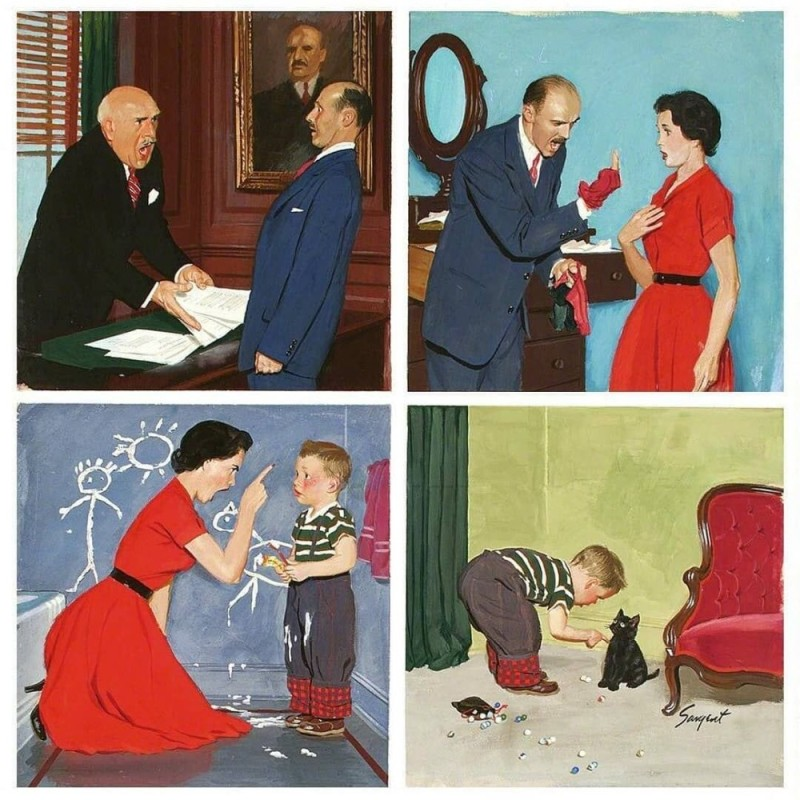
\includegraphics[width=\textwidth]{Report/pics/cycle of abuse.png}
        \caption{Inspirational diagram for forming a scientific question.}
        \label{fig:cycle-of-abuse}
    \end{subfigure}
    \hfill
    \begin{subfigure}[t]{0.48\textwidth}
        \centering
        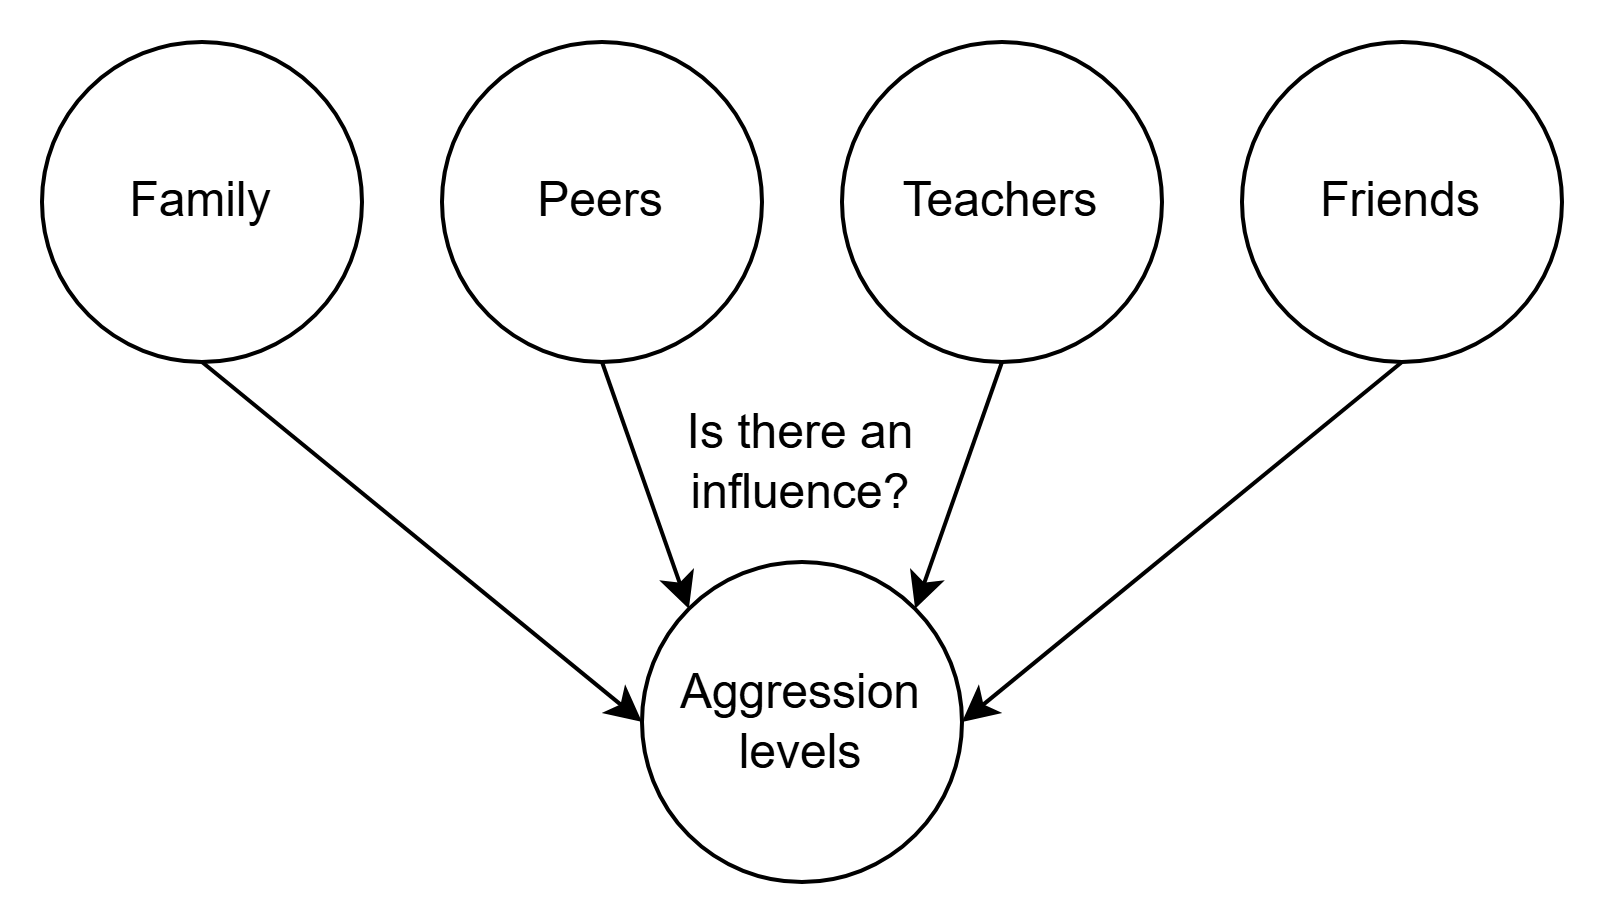
\includegraphics[width=\textwidth]{Report/pics/scheme for scientific question.png}
        \caption{Conceptual scheme illustrating the scientific question.}
        \label{fig:scientific-question}
    \end{subfigure}
    \caption{The first figure serves as inspiration, while the second is a vague schematic formulation of our scientific question.}
    \label{fig:question-figures}
\end{figure}

\section{Selected Algorithm}
\label{sec:algorithm}

\subsection{Algorithm Description}
[Describe the FCI algorithm: inputs, outputs (PAG), and how it works using conditional independence tests.]

\subsection{Assumptions}
[Explain assumptions like causal sufficiency (not required for FCI), faithfulness, and correctness of the conditional independence tests.]

\subsection{Advantages and Limitations}
[Discuss strengths (e.g., handles latent confounding) and challenges (e.g., complexity, sensitivity to CI test errors).]

\subsection{Graph Type}
[Explain that FCI estimates a Partial Ancestral Graph (PAG), allowing for bi-directed and circle-ended edges to account for hidden variables.]



\section{Methodology}
\label{sec:methodology}

\subsection{Causal Discovery Setup}
[Explain the full pipeline: preprocessing → conditional independence tests → FCI execution → graph extraction.]

\subsection{Parameter Choices}
[Describe the independence test (e.g., G² test or Fisher's Z), significance level (e.g., $\alpha = 0.05$), and library used (e.g., `causal-learn` in Python).]

\subsection{Software and Implementation}
[Specify tools used: Python, causal-learn, pandas, numpy, matplotlib. Optionally show code snippets.]

\section{Results}
\label{sec:results}

\subsection{Learned Causal Structure}
[Include your graph as a figure.]

% \begin{figure}[h]
% \centering
% \includegraphics[width=0.8\textwidth]{fci_result.png}
% \caption{Learned PAG using FCI algorithm on HBSC 2018 subset.}
% \label{fig:fci_graph}
% \end{figure}

\subsection{Interpretation}
[Explain notable relationships (e.g., parental communication → peer trust → life satisfaction). Which arrows suggest direct influence? Where are bidirected edges?]

\subsection{Sensitivity to Parameters}
[Optionally, mention results under different $\alpha$ values, sample sizes, or independence tests.]

\section{Discussion}
\label{sec:discussion}

\begin{itemize}
    \item Are the discovered causal paths meaningful and interpretable?
    \item What are the limitations of this approach given the observational nature of HBSC?
    \item Are the assumptions of the FCI algorithm likely to hold in this case?
    \item Could latent variables (e.g., personality traits) explain some of the results?
\end{itemize}

\section{Conclusion}
\label{sec:conclusion}

[Summarize the main contributions: application of FCI to HBSC data, handling challenges of mixed data and confounding, and interpretation of the resulting PAG. Mention possible future work, such as testing other algorithms (e.g., GES) or estimating causal effects using IDA.]

\begin{thebibliography}{9}
\bibitem{pearl2009causality}
  Judea Pearl,
  \emph{Causality: Models, Reasoning and Inference}.
  Cambridge University Press, 2009.

\bibitem{spirtes2000causation}
  Peter Spirtes, Clark Glymour, and Richard Scheines,
  \emph{Causation, Prediction, and Search}.
  MIT Press, 2000.

\bibitem{zheng2018dags}
  Xun Zheng et al.,
  \emph{DAGs with NO TEARS: Continuous Optimization for Structure Learning}.
  NeurIPS, 2018.

\bibitem{glymour2019review}
  Clark Glymour, Kun Zhang, and Peter Spirtes,
  \emph{Review of causal discovery methods based on graphical models}.
  Frontiers in Genetics, 10 (2019): 524.
\end{thebibliography}

\begin{appendices}
\section{Variables description}
\label{appendix:missing_values_table}
\begin{table}[htbp]

\centering
\tiny{
\begin{tabular}{lrrrrrrrrr} 
\scriptsize

% \toprule
Variable & N & Mean & SD & Min & P25 & P50 & P75 & Max & Missing \\
\midrule
lifesat & 239585 & 7.739& 1.927& 0.000& 7.000& 8.000& 9.000& 10.000& 4512 \\
irritable & 237558 & 3.505& 1.357& 1.000& 2.000& 4.000& 5.000& 5.000& 6539 \\
nervous & 237572 & 3.545& 1.390& 1.000& 2.000& 4.000& 5.000& 5.000& 6525 \\
fmeal & 229359 & 1.803& 1.021& 1.000& 1.000& 2.000& 2.000& 5.000& 14738 \\
timeexe & 239298 & 3.035& 1.646& 1.000& 2.000& 3.000& 4.000& 7.000& 4799 \\
friendhelp & 234353 & 5.164& 1.925& 1.000& 4.000& 6.000& 7.000& 7.000& 9744 \\
friendcounton & 233723 & 5.239& 1.956& 1.000& 4.000& 6.000& 7.000& 7.000& 10374 \\
friendshare & 233284 & 5.468& 1.957& 1.000& 4.000& 6.000& 7.000& 7.000& 10813 \\
friendtalk & 233289 & 5.166& 2.069& 1.000& 4.000& 6.000& 7.000& 7.000& 10808 \\
likeschool & 238988 & 2.080& 0.895& 1.000& 1.000& 2.000& 3.000& 4.000& 5109 \\
schoolpressure & 238611 & 2.287& 0.944& 1.000& 2.000& 2.000& 3.000& 4.000& 5486 \\
studtogether & 227746 & 2.146& 0.991& 1.000& 1.000& 2.000& 3.000& 5.000& 16351 \\
studhelpful & 227351 & 2.266& 1.056& 1.000& 1.000& 2.000& 3.000& 5.000& 16746 \\
studaccept & 226653 & 2.044& 1.041& 1.000& 1.000& 2.000& 3.000& 5.000& 17444 \\
teacheraccept & 227333 & 1.916& 0.975& 1.000& 1.000& 2.000& 2.000& 5.000& 16764 \\
teachercare & 225757 & 2.295& 1.083& 1.000& 1.000& 2.000& 3.000& 5.000& 18340 \\
teachertrust & 226258 & 2.317& 1.165& 1.000& 1.000& 2.000& 3.000& 5.000& 17839 \\
bulliedothers & 222518 & 1.327& 0.776& 1.000& 1.000& 1.000& 1.000& 5.000& 21579 \\
beenbullied & 227135 & 1.475& 0.969& 1.000& 1.000& 1.000& 2.000& 5.000& 16962 \\
cbulliedothers & 229163 & 1.159& 0.581& 1.000& 1.000& 1.000& 1.000& 5.000& 14934 \\
cbeenbullied & 229013 & 1.208& 0.641& 1.000& 1.000& 1.000& 1.000& 5.000& 15084 \\
fight12m & 235335 & 1.717& 1.195& 1.000& 1.000& 1.000& 2.000& 5.000& 8762 \\
injured12m & 235123 & 1.814& 1.158& 1.000& 1.000& 1.000& 2.000& 5.000& 8974 \\
emconlfreq1 & 217377 & 4.207& 1.568& 1.000& 3.000& 4.000& 6.000& 6.000& 26720 \\
emconlfreq2 & 214545 & 3.473& 1.556& 1.000& 2.000& 3.000& 5.000& 6.000& 29552 \\
emconlfreq3 & 215124 & 2.376& 1.500& 1.000& 1.000& 2.000& 3.000& 6.000& 28973 \\
emconlfreq4 & 215094 & 3.445& 1.625& 1.000& 2.000& 3.000& 5.000& 6.000& 29003 \\
emconlpref1 & 214284 & 7.358& 21.618& 1.000& 1.000& 2.000& 3.000& 99.000& 29813 \\
emconlpref2 & 213511 & 7.458& 21.636& 1.000& 1.000& 2.000& 4.000& 99.000& 30586 \\
emconlpref3 & 213& 7.395& 21.677& 1.000& 1.000& 2.000& 3.000& 99.000& 31097 \\
emcsocmed1 & 212124 & 6.410& 21.925& 1.000& 1.000& 1.000& 2.000& 99.000& 31973 \\
emcsocmed2 & 212438 & 6.373& 21.916& 1.000& 1.000& 1.000& 1.000& 99.000& 31659 \\
emcsocmed3 & 212088 & 6.405& 21.928& 1.000& 1.000& 1.000& 2.000& 99.000& 32009 \\
emcsocmed4 & 211669 & 6.505& 21.928& 1.000& 1.000& 1.000& 2.000& 99.000& 32428 \\
emcsocmed5 & 211654 & 6.362& 21.961& 1.000& 1.000& 1.000& 1.000& 99.000& 32443 \\
emcsocmed6 & 211553 & 6.394& 21.959& 1.000& 1.000& 1.000& 1.000& 99.000& 32544 \\
emcsocmed7 & 211500 & 6.355& 21.971& 1.000& 1.000& 1.000& 1.000& 99.000& 32597 \\
emcsocmed8 & 211219 & 6.518& 21.950& 1.000& 1.000& 1.000& 2.000& 99.000& 32878 \\
emcsocmed9 & 211242 & 6.360& 21.984& 1.000& 1.000& 1.000& 1.000& 99.000& 32855 \\
motherhome1 & 233862 & 1.073& 0.260& 1.000& 1.000& 1.000& 1.000& 2.000& 10235 \\
fatherhome1 & 233934 & 1.272& 0.445& 1.000& 1.000& 1.000& 2.000& 2.000& 10163 \\
stepmohome1 & 233648 & 1.979& 0.144& 1.000& 2.000& 2.000& 2.000& 2.000& 10449 \\
stepfahome1 & 233646 & 1.941& 0.236& 1.000& 2.000& 2.000& 2.000& 2.000& 10451 \\
fosterhome1 & 233159 & 1.991& 0.097& 1.000& 2.000& 2.000& 2.000& 2.000& 10938 \\
elsehome1\_2 & 232973 & 1.801& 0.399& 1.000& 2.000& 2.000& 2.000& 2.000& 11124 \\
employfa & 220098 & 1.202& 0.643& 1.000& 1.000& 1.000& 1.000& 4.000& 23999 \\
employmo & 219962 & 1.243& 0.502& 1.000& 1.000& 1.000& 1.000& 4.000& 24135 \\
employnotfa & 19573 & 2.673& 1.245& 1.000& 1.000& 3.000& 4.000& 4.000& 224524 \\
employnotmo & 44207 & 2.775& 0.925& 1.000& 2.000& 3.000& 3.000& 4.000& 199890 \\
talkfather & 226606 & 2.221& 1.180& 1.000& 1.000& 2.000& 3.000& 5.000& 17491 \\
talkstepfa & 177072 & 4.455& 1.141& 1.000& 5.000& 5.000& 5.000& 5.000& 67025 \\
talkmother & 228576 & 1.738& 0.939& 1.000& 1.000& 1.000& 2.000& 5.000& 15521 \\
talkstepmo & 175091 & 4.556& 1.055& 1.000& 5.000& 5.000& 5.000& 5.000& 69006 \\
famhelp & 225201 & 5.835& 1.866& 1.000& 5.000& 7.000& 7.000& 7.000& 18896 \\
famsup & 224006 & 5.669& 1.912& 1.000& 5.000& 7.000& 7.000& 7.000& 20091 \\
famtalk & 224078 & 5.424& 2.015& 1.000& 4.000& 6.000& 7.000& 7.000& 20019 \\
famdec & 223860 & 5.723& 1.884& 1.000& 5.000& 7.000& 7.000& 7.000& 20237 \\
MBMI & 190786 & 19.507& 3.682& 0.000& 17.087& 19.044& 21.403& 44.911& 53311 \\
IRFAS & 231498 & 7.892& 2.770& 0.000& 6.000& 8.000& 10.000& 13.000& 12599 \\
IRRELFAS\_LMH & 231498 & 1.990& 0.621& 1.000& 2.000& 2.000& 2.000& 3.000& 12599 \\
id1 & 244097 & 15.044& 75.535& 1.000& 1.000& 5.000& 12.000& 999.000& 0 \\
id2 & 244097 & 262.459& 843.224& 1.000& 41.000& 98.000& 199.000& 9999.000& 0 \\
id3 & 223290 & 1588.415& 6113.380& 1.000& 102.000& 215.000& 472.000& 85701.000& 20807 \\
id4 & 244097 & 158298.700& 768215.441& 1.000& 1856.000& 3818.000& 7996.000& 5244023.000& 0 \\
adm & 244097 & 1.452& 0.498& 1.000& 1.000& 1.000& 2.000& 2.000& 0 \\
month & 244079 & 5.493& 3.250& 1.000& 3.000& 5.000& 6.000& 12.000& 18 \\
age & 242581 & 13.498& 1.629& 10.000& 11.833& 13.500& 15.167& 16.500& 1516 \\
sex & 244097 & 1.507& 0.500& 1.000& 1.000& 2.000& 2.000& 2.000& 0 \\
grade & 179267 & 1.973& 0.810& 1.000& 1.000& 2.000& 3.000& 3.000& 64830 \\
\bottomrule
\end{tabular}
\caption{Summary statistics of all selected variables.}
\end{table}}


\end{appendices}
\end{document}
